\documentclass[tikz, border=3pt]{standalone}

\usepackage{amsmath,amssymb}
\usepackage{pgfplots}
\pgfplotsset{compat=1.18}
\usepgfplotslibrary{groupplots}
\usetikzlibrary{arrows.meta}
\usepackage{xcolor}

\definecolor{utnblue}{RGB}{0, 51, 102}
\definecolor{utnred}{RGB}{204, 0, 0}

\pgfplotsset{
    panelzn/.style={
        axis lines=middle,
        width=6.4cm, height=5cm,
        xmin=-0.6, xmax=6.2,
        xtick={0,1,2,3,4,5,6},
        tick label style={font=\tiny},
        label style={font=\scriptsize},
        title style={font=\scriptsize, at={(axis description cs:1,1)},
                     anchor=north east, xshift=-2pt, yshift=-2pt},
        xticklabel style={fill=white, inner sep=1.5pt},
        every axis x label/.style={at={(ticklabel* cs:1)}, anchor=west},
        every axis y label/.style={at={(ticklabel* cs:1)}, anchor=south},
        enlargelimits=false,
        clip mode=individual,
        xlabel={$n$},
    },
}

\begin{document}
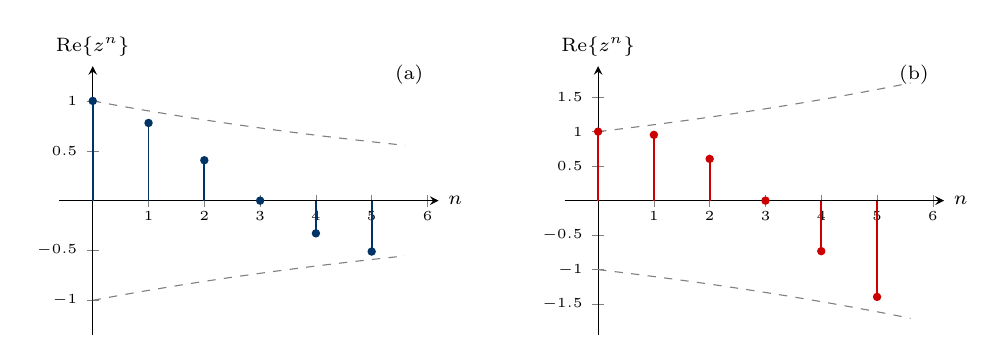
\begin{tikzpicture}[font=\scriptsize]

\begin{groupplot}[
    group style={group size=2 by 1, horizontal sep=1.6cm},
    panelzn,
]

% ---------------- (a) r = 0,9 ----------------
\nextgroupplot[title={(a)}, ymin=-1.35, ymax=1.35, ytick={-1,-0.5,0.5,1},
               ylabel={$\operatorname{Re}\{z^n\}$}]
\addplot[gray, dashed, thin, domain=0:5.6, samples=40] {0.9^x};
\addplot[gray, dashed, thin, domain=0:5.6, samples=40] {-0.9^x};
\addplot[ycomb, utnblue, semithick, mark=*, mark size=1.2pt,
         mark options={fill=utnblue, draw=utnblue}]
    coordinates {(0,1) (1,0.779) (2,0.405) (3,0) (4,-0.328) (5,-0.511)};

% ---------------- (b) r = 1,1 ----------------
\nextgroupplot[title={(b)}, ymin=-1.95, ymax=1.95, ytick={-1.5,-1,-0.5,0.5,1,1.5},
               ylabel={$\operatorname{Re}\{z^n\}$}]
\addplot[gray, dashed, thin, domain=0:5.6, samples=40] {1.1^x};
\addplot[gray, dashed, thin, domain=0:5.6, samples=40] {-1.1^x};
\addplot[ycomb, utnred, semithick, mark=*, mark size=1.2pt,
         mark options={fill=utnred, draw=utnred}]
    coordinates {(0,1) (1,0.953) (2,0.605) (3,0) (4,-0.732) (5,-1.395)};

\end{groupplot}

\end{tikzpicture}
\end{document}
